%%%%%%%%%%%%%%%%%%%%%%%%%%%%%%%%%%%%%%%%%
% Appendix
% 
% $Date$
% $Rev$:
% $Author$


\appendix
\chapter{Appendix}

  \section{Additional Source Code Listings}
    \subsection{MyNamedPipeManager and MyPipe}
      \setJavaCodeListing
      \lstinputlisting[caption=MyNamedPipeManager.java]{\customComponentsBookstoreApplicationDir/src/bookstoreTracing/MyNamedPipeManager.java}

      \setJavaCodeListing
      \lstinputlisting[caption=MyPipe.java]{\customComponentsBookstoreApplicationDir/src/bookstoreTracing/MyPipe.java}

\newpage
  \section{Example File System Monitoring Logs}

	\subsection{Chapter \ref{chap:example}}
		The following listing shows the produced log during a run of the Bookstore Application with the manual monitoring probes.
		\setTextListing
\begin{lstlisting}[caption=Execution of the manually instrumented Bookstore application (Section~\ref{sec:example:monitoring})]
Apr 28, 2011 5:15:25 PM kieker.monitoring.core.configuration.Configuration createSingletonConfiguration
INFO: Loading properties from properties file in classpath: 'META-INF/kieker.monitoring.properties'
Apr 28, 2011 5:15:25 PM kieker.monitoring.core.configuration.Configuration loadConfigurationFromResource
WARNING: File 'META-INF/kieker.monitoring.properties' not found in classpath
Apr 28, 2011 5:15:25 PM kieker.monitoring.core.controller.MonitoringController createInstance
INFO: Current State of kieker.monitoring (1.3-20110427) Status: 'enabled'
	Name: 'KIEKER-SINGLETON'; Hostname: 'Kaapstad'; experimentID: '1'
WriterController:
	Number of Inserts: '0'
	Automatic assignment of logging timestamps: 'true'
Writer: 'kieker.monitoring.writer.filesystem.AsyncFsWriter'
	Configuration:
		kieker.monitoring.writer.filesystem.AsyncFsWriter.QueueFullBehavior='0'
		kieker.monitoring.writer.filesystem.AsyncFsWriter.QueueSize='10000'
		kieker.monitoring.writer.filesystem.AsyncFsWriter.customStoragePath=''
		kieker.monitoring.writer.filesystem.AsyncFsWriter.storeInJavaIoTmpdir='true'
	Writer Threads (1): 
		Finished: 'false'; Writing to Directory: '/tmp/kieker-20110428-151525684-UTC-Kaapstad-KIEKER-SINGLETON'
Sampling Controller: Periodic Sensor available: Current Poolsize: '0'; Scheduled Tasks: '0'
Bookstore.main: Starting request 0
Bookstore.main: Starting request 1
Apr 28, 2011 5:15:25 PM kieker.monitoring.writer.filesystem.MappingFileWriter writeMapping
INFO: Registered monitoring record type with id '1':kieker.common.record.OperationExecutionRecord
Bookstore.main: Starting request 2
Bookstore.main: Starting request 3
Bookstore.main: Starting request 4
\end{lstlisting}

		The second listing is the log during the analysis of the produced data. It can be seen that some of the calls are accepted and some others refused.
		\setTextListing
\begin{lstlisting}[caption=Execution of the example analysis (Section~\ref{sec:example:analysis})]
19.08.2010 13:19:55 kieker.analysis.AnalysisController registerPlugin
INFO: Registered plugin bookstoreApplication.Consumer@6ac2a132
19.08.2010 13:19:55 kieker.analysis.AnalysisController registerPlugin
INFO: Plugin bookstoreApplication.Consumer@6ac2a132 also registered as record consumer
19.08.2010 13:19:55 kieker.analysis.reader.filesystem.FSDirectoryReader processInputFile
INFO: < Loading C:\Temp\tpmon-20100814-103954167-UTC\tpmon-20100814-103954184-UTC-Thread-2.dat
19.08.2010 13:19:55 kieker.common.record.MonitoringRecordTypeRegistry registerRecordTypeIdMapping
INFO: Registered record type mapping 1/kieker.common.record.OperationExecutionRecord
maximal response time exceeded by 11382559 ns: bookstoreApplication.Catalog.getBook()
maximal response time exceeded by 11251720 ns: bookstoreApplication.Catalog.getBook()
maximal response time exceeded by 80320 ns: bookstoreApplication.Catalog.getBook()
maximal response time exceeded by 27400 ns: bookstoreApplication.Catalog.getBook()
maximal response time exceeded by 81760 ns: bookstoreApplication.Catalog.getBook()
maximal response time exceeded by 24240 ns: bookstoreApplication.Catalog.getBook()
maximal response time exceeded by 82480 ns: bookstoreApplication.Catalog.getBook()
response time accepted: bookstoreApplication.Catalog.getBook()
response time accepted: bookstoreApplication.Catalog.getBook()
response time accepted: bookstoreApplication.Catalog.getBook()
14.08.2010 12:41:02 kieker.analysis.reader.filesystem.FSReader$\$$FSReaderCons execute
INFO: All reader threads provided FS_READER_TERMINATION_MARKER
\end{lstlisting}
	
	\subsection{Chapter \ref{chap:aspectJ}}
	    The following listing shows the produced log during a run of the Bookstore Application, weaved with the necessary code at runtime as shown in Section \ref{sec:aspectJ:fullweaving}.
		\setTextListing
\begin{lstlisting}[caption=Execution of the Bookstore with AspectJ trace instrumentation (Section~\ref{sec:traceAnalysis:instr:AspectJ})]
Bookstore.main: Starting request 0
Apr 28, 2011 4:28:29 PM kieker.monitoring.core.configuration.Configuration createSingletonConfiguration
INFO: Loading properties from properties file in classpath: 'META-INF/kieker.monitoring.properties'
Apr 28, 2011 4:28:29 PM kieker.monitoring.core.controller.MonitoringController createInstance
INFO: Current State of kieker.monitoring (1.3-20110427) Status: 'enabled'
	Name: 'KIEKER'; Hostname: 'Kaapstad'; experimentID: '1'
WriterController:
	Number of Inserts: '0'
	Automatic assignment of logging timestamps: 'true'
Writer: 'kieker.monitoring.writer.filesystem.AsyncFsWriter'
	Configuration:
		kieker.monitoring.writer.filesystem.AsyncFsWriter.QueueFullBehavior='0'
		kieker.monitoring.writer.filesystem.AsyncFsWriter.QueueSize='10000'
		kieker.monitoring.writer.filesystem.AsyncFsWriter.customStoragePath=''
		kieker.monitoring.writer.filesystem.AsyncFsWriter.storeInJavaIoTmpdir='true'
	Writer Threads (1): 
		Finished: 'false'; Writing to Directory: '/tmp/kieker-20110428-142829399-UTC-Kaapstad-KIEKER'
Sampling Controller: Periodic Sensor available: Current Poolsize: '0'; Scheduled Tasks: '0'
Apr 28, 2011 4:28:29 PM kieker.monitoring.core.registry.ControlFlowRegistry <init>
INFO: First threadId will be 7752665283541598209
Apr 28, 2011 4:28:29 PM kieker.monitoring.writer.filesystem.MappingFileWriter writeMapping
INFO: Registered monitoring record type with id '1':kieker.common.record.OperationExecutionRecord
\end{lstlisting}



	
\newpage
  \section{Ant Scripts}
    \subsection{Chapter \ref{chap:example}}
      Following listings show the necessary \file{build.xml} and \file{build.properties} to compile and execute the manual instrumentated Bookstore Application shown in Chapter~\ref{chap:example}.
      \setXMLListing
      \lstinputlisting[caption=build.xml]{\manualInstrumentedBookstoreApplicationDir/build.xml}
      \lstinputlisting[caption=build.properties]{\manualInstrumentedBookstoreApplicationDir/build.properties}
      In order to run the analysis of the application, it is still necessary to supply the program with the path to the output directory of the monitoring. This is done via the parameter "analysis.directory", e.g.:
      \setBashListing
      \begin{lstlisting}[caption=Command to compile and run the instrumented Bookstore via ant]
#\lstshellprompt{}# ant run-analysis -Danalysis.directory /tmp/kicker-20120402-163314855-UTC-myHost-KIEKER-SINGLETON
\end{lstlisting}%-KIEKER


    \subsection{Chapter \ref{chap:componentsMonitoring} and \ref{chap:componentsAnalysis}}
      Following listings show the necessary \file{build.xml} and \file{build.properties} to compile and execute the manually instrumentated Bookstore Application with the own components shown in Chapter~\ref{chap:componentsMonitoring} and \ref{chap:componentsAnalysis}.
      \setXMLListing
      \lstinputlisting[caption=build.xml]{\customComponentsBookstoreApplicationDir/build.xml}
      \lstinputlisting[caption=build.properties]{\customComponentsBookstoreApplicationDir/build.properties}

    \subsection{Chapter \ref{chap:aspectJ}}
      Following listings show the necessary \file{build.xml} and \file{build.properties} to compile and execute the Bookstore Application instrumentated with AspectJ shown in Chapter~\ref{chap:aspectJ}.
      \setXMLListing
      \lstinputlisting[caption=build.xml]{\aspectJBookstoreApplicationDir/build.xml}
      \lstinputlisting[caption=build.properties]{\aspectJBookstoreApplicationDir/build.properties}     

\newpage
  \section{Example Graphs and Diagrams}
    \begin{figure}[h]\centering
	\subfigure[]{\label{fig:appendix:aggregatedAllocationCallTree}%
	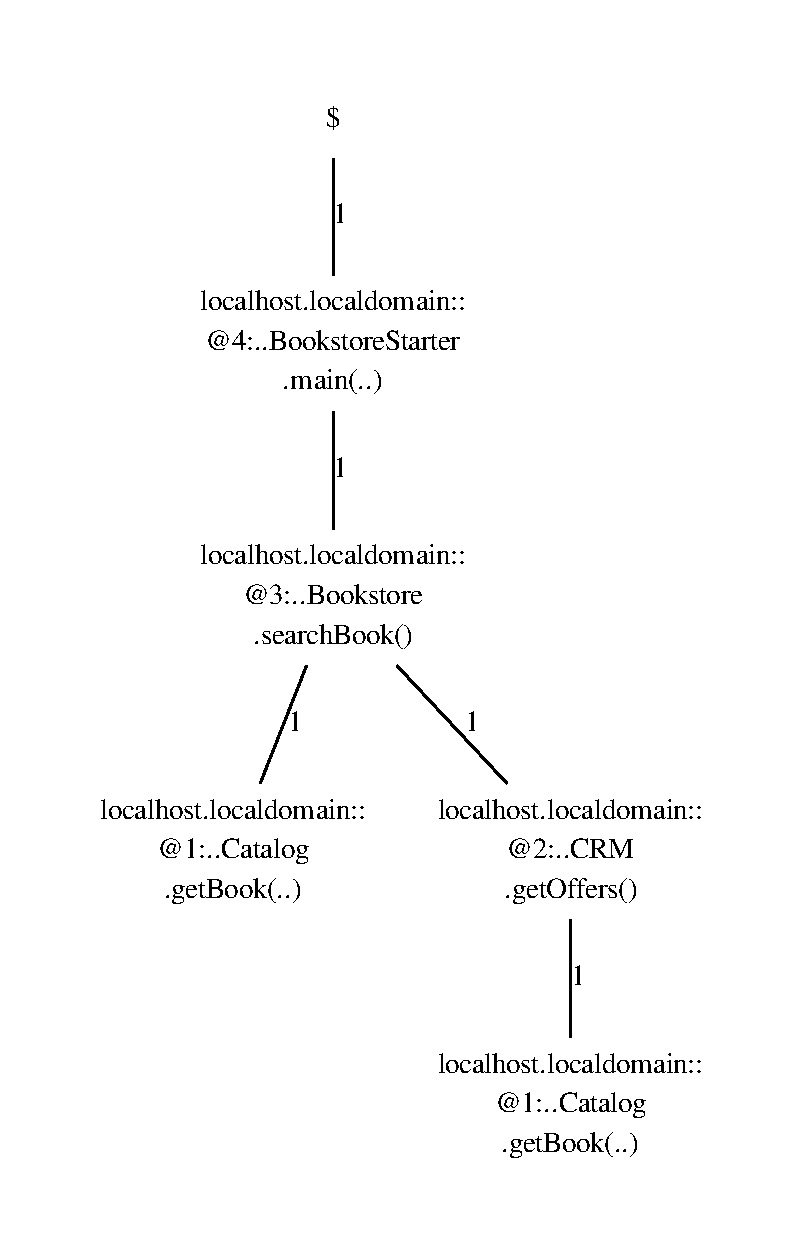
\includegraphics[width=0.33\textwidth]{images/aggregatedAllocationCallTree}%
	}%
	\subfigure[]{\label{fig:appendix:aggregatedAssemblyCallTree}%
	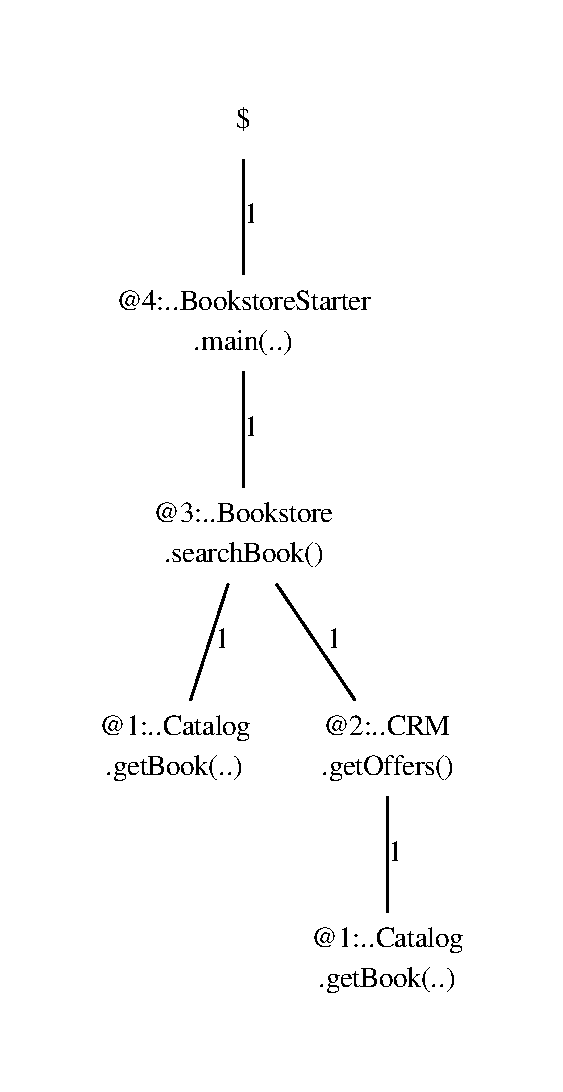
\includegraphics[width=0.33\textwidth]{images/aggregatedAssemblyCallTree}%
	}%
	\subfigure[]{\label{fig:appendix:callTree}%
	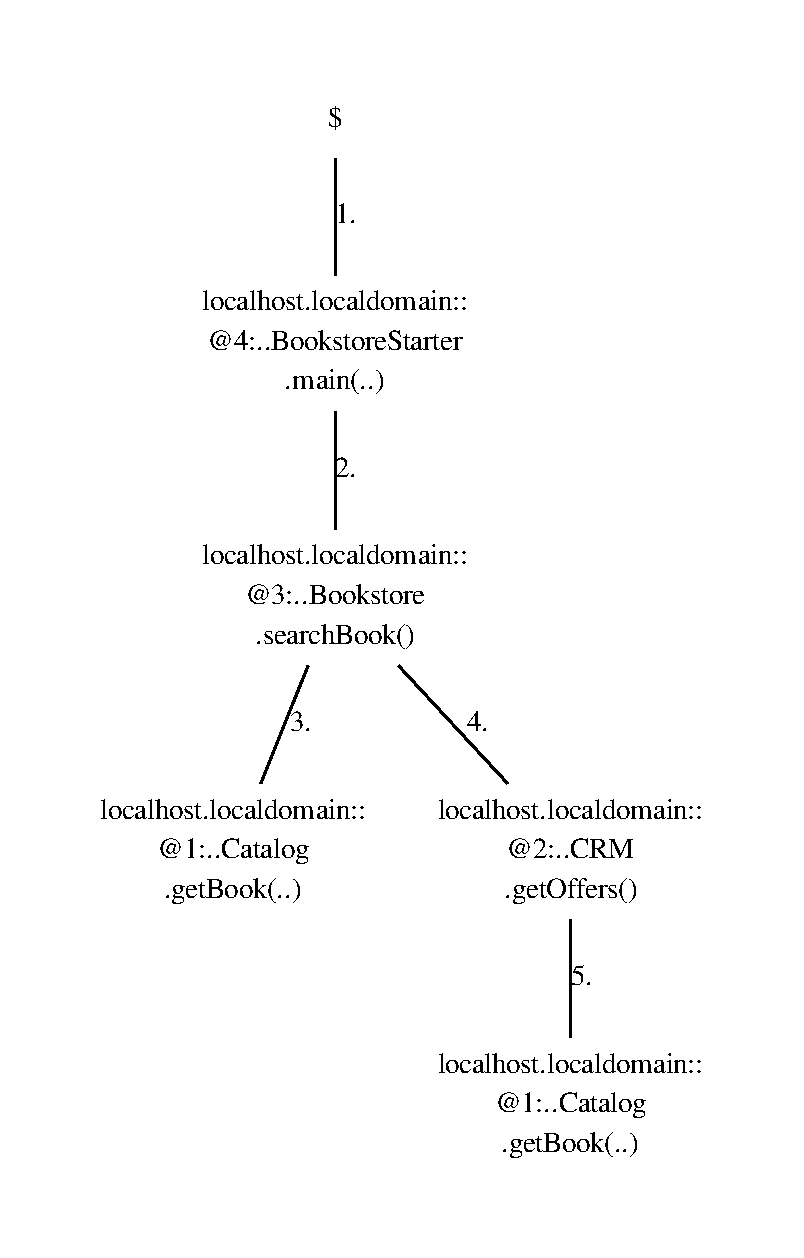
\includegraphics[width=0.33\textwidth]{images/callTree}%
	}%
	\caption{Aggregated Allocation Call Tree~\subref{fig:appendix:aggregatedAllocationCallTree}, Aggregated Assembly Call Tree~\subref{fig:appendix:aggregatedAssemblyCallTree} and Call Tree~\subref{fig:appendix:callTree}}
	\end{figure}
	
	\begin{figure}[H]
		\centering
		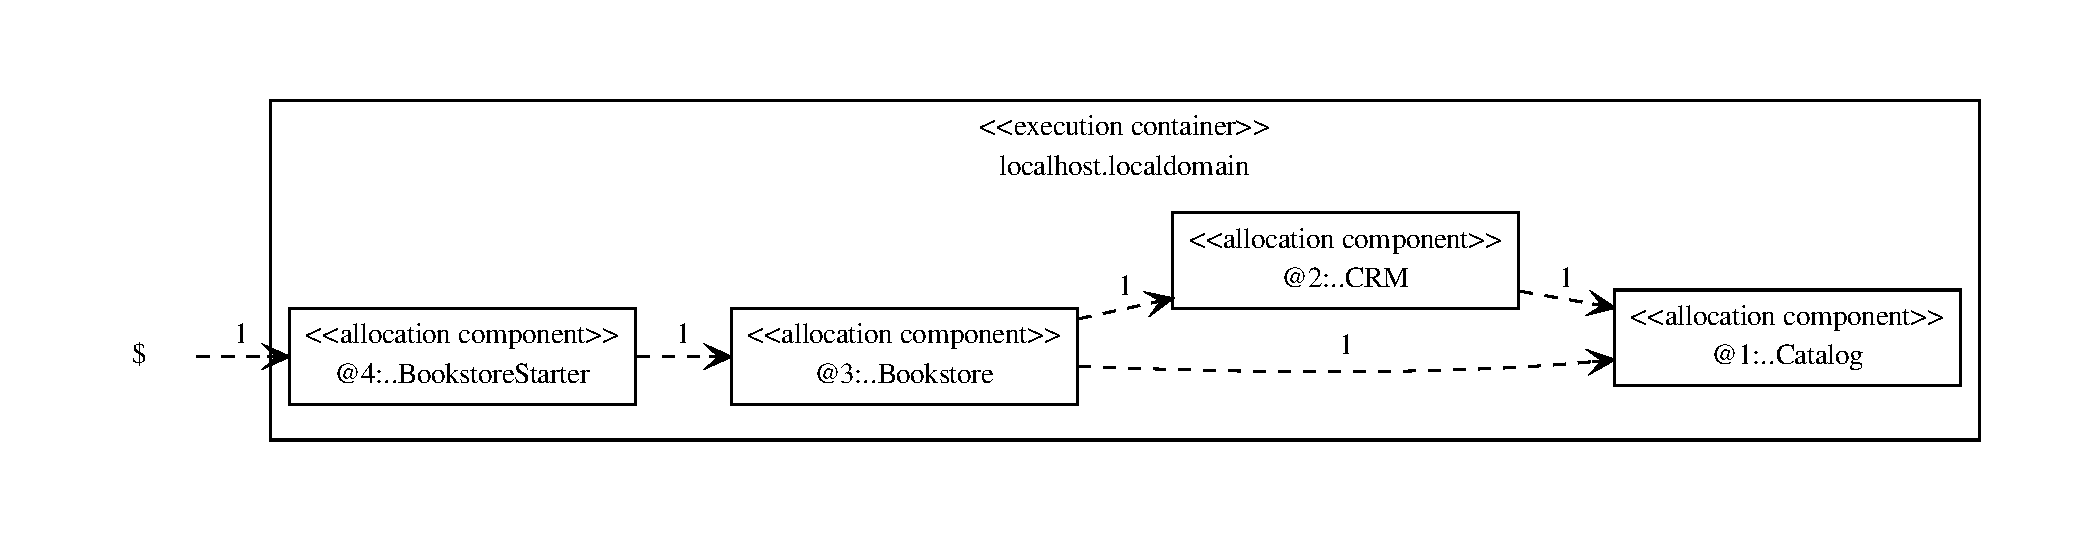
\includegraphics[width=1.0\textwidth]{images/allocationComponentDependencyGraph}
		\caption{allocationComponentDependencyGraph}
	\end{figure}
	\begin{figure}[H]
		\centering
		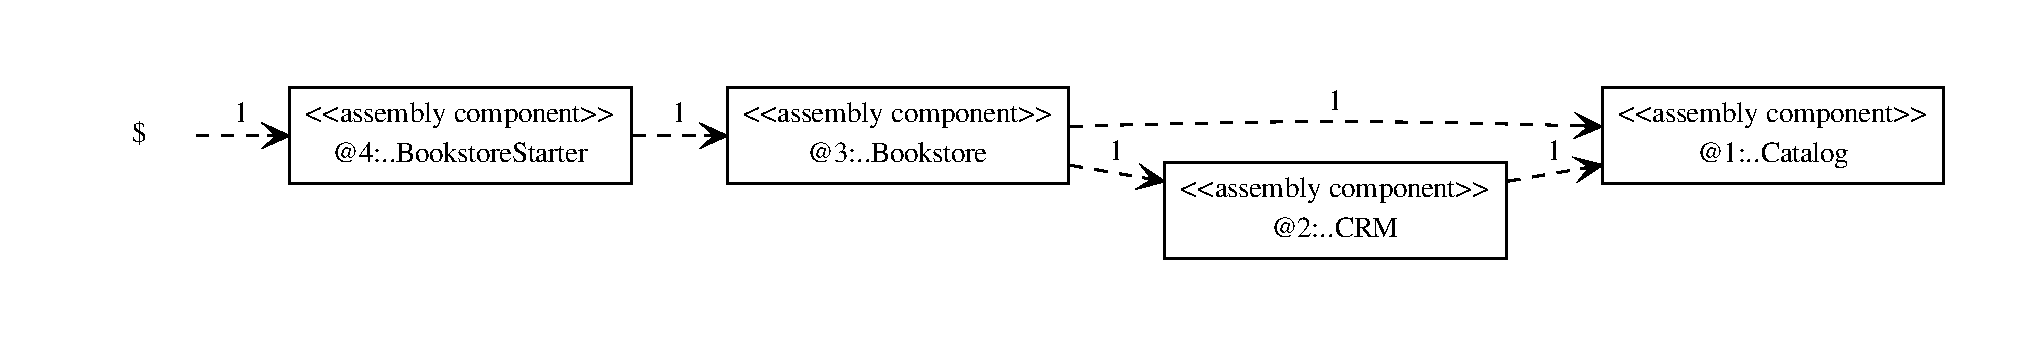
\includegraphics[width=1.0\textwidth]{images/assemblyComponentDependencyGraph}
		\caption{assemblyComponentDependencyGraph}
	\end{figure}
	
	\begin{figure}[H]
		\centering
		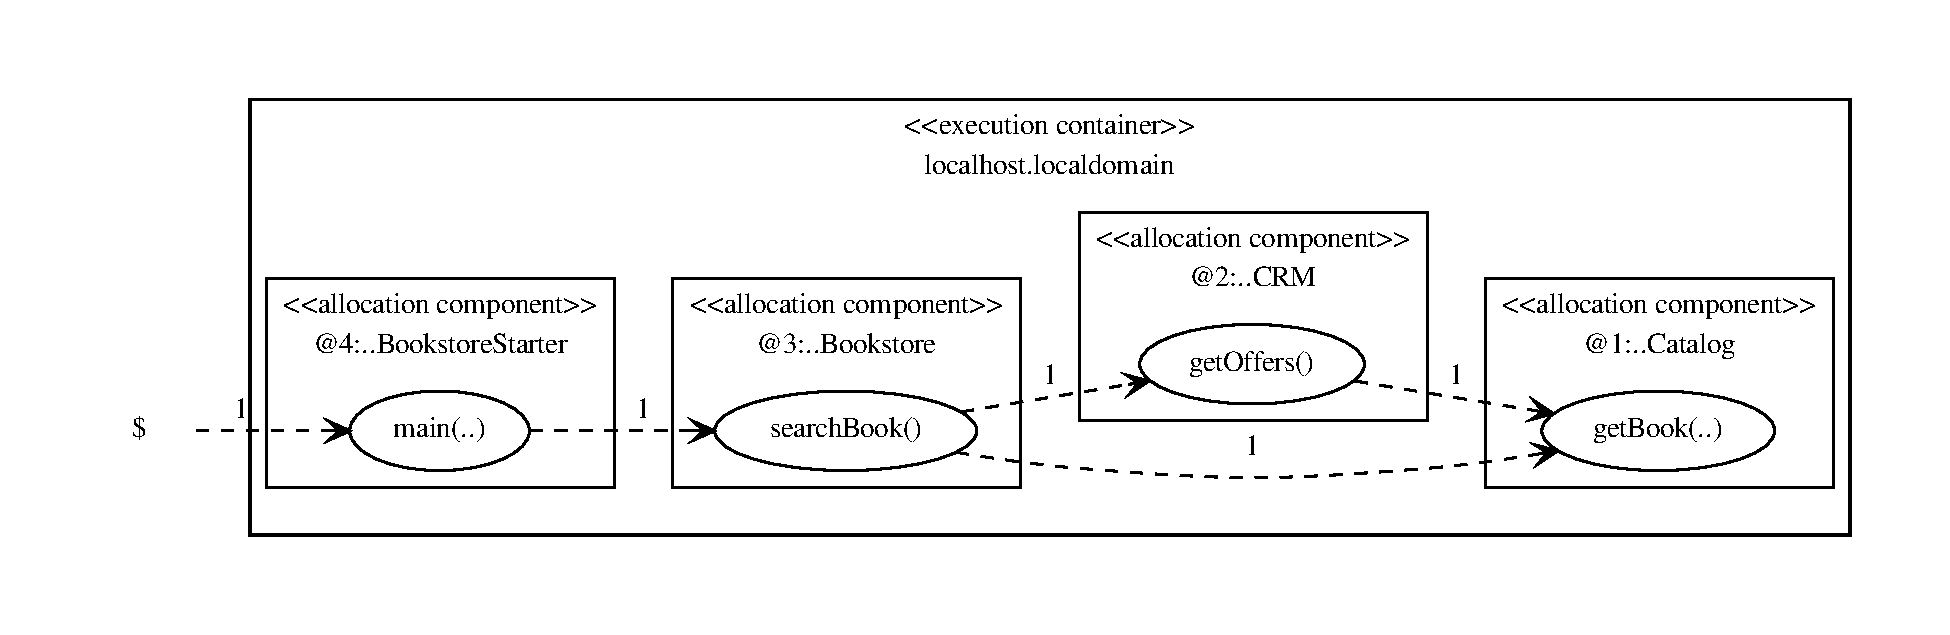
\includegraphics[width=1.0\textwidth]{images/allocationOperationDependencyGraph}
		\caption{allocationOperationDependencyGraph}
	\end{figure}
	\begin{figure}[H]
		\centering
		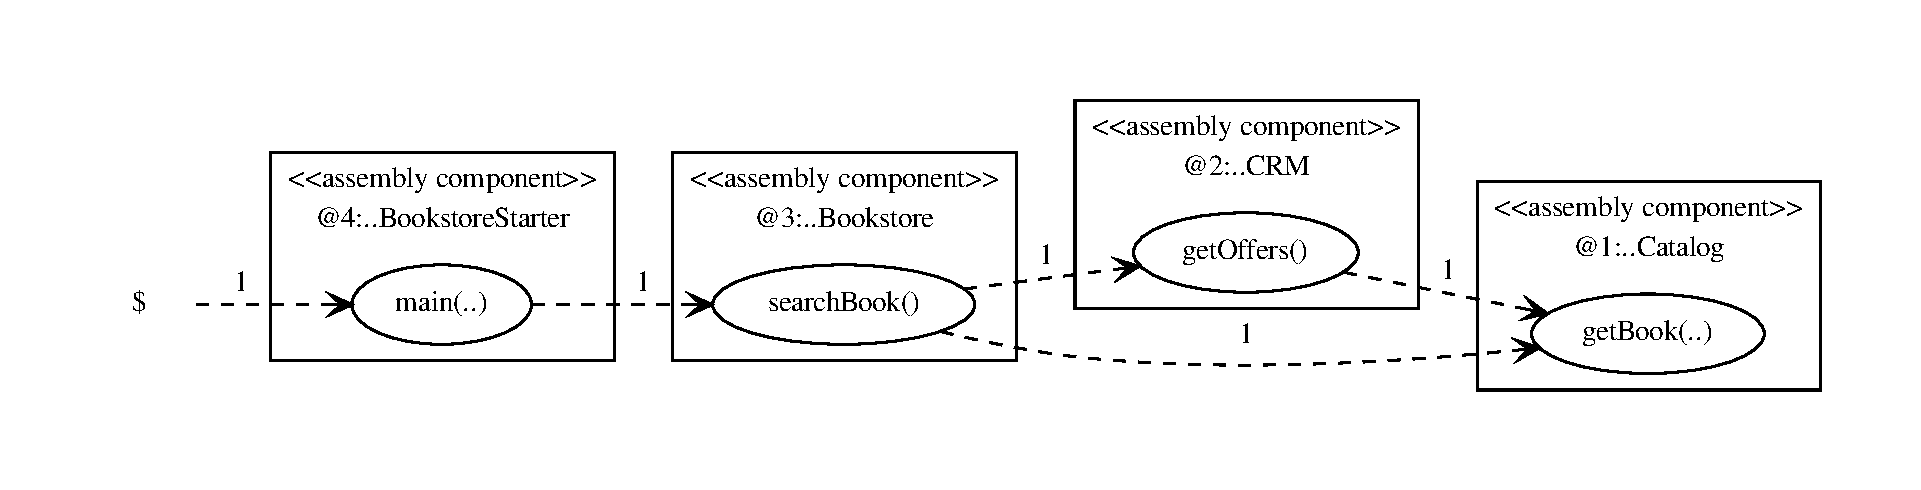
\includegraphics[width=1.0\textwidth]{images/assemblyOperationDependencyGraph}
		\caption{assemblyOperationDependencyGraph}
	\end{figure}
	
	\begin{figure}[H]
		\centering
		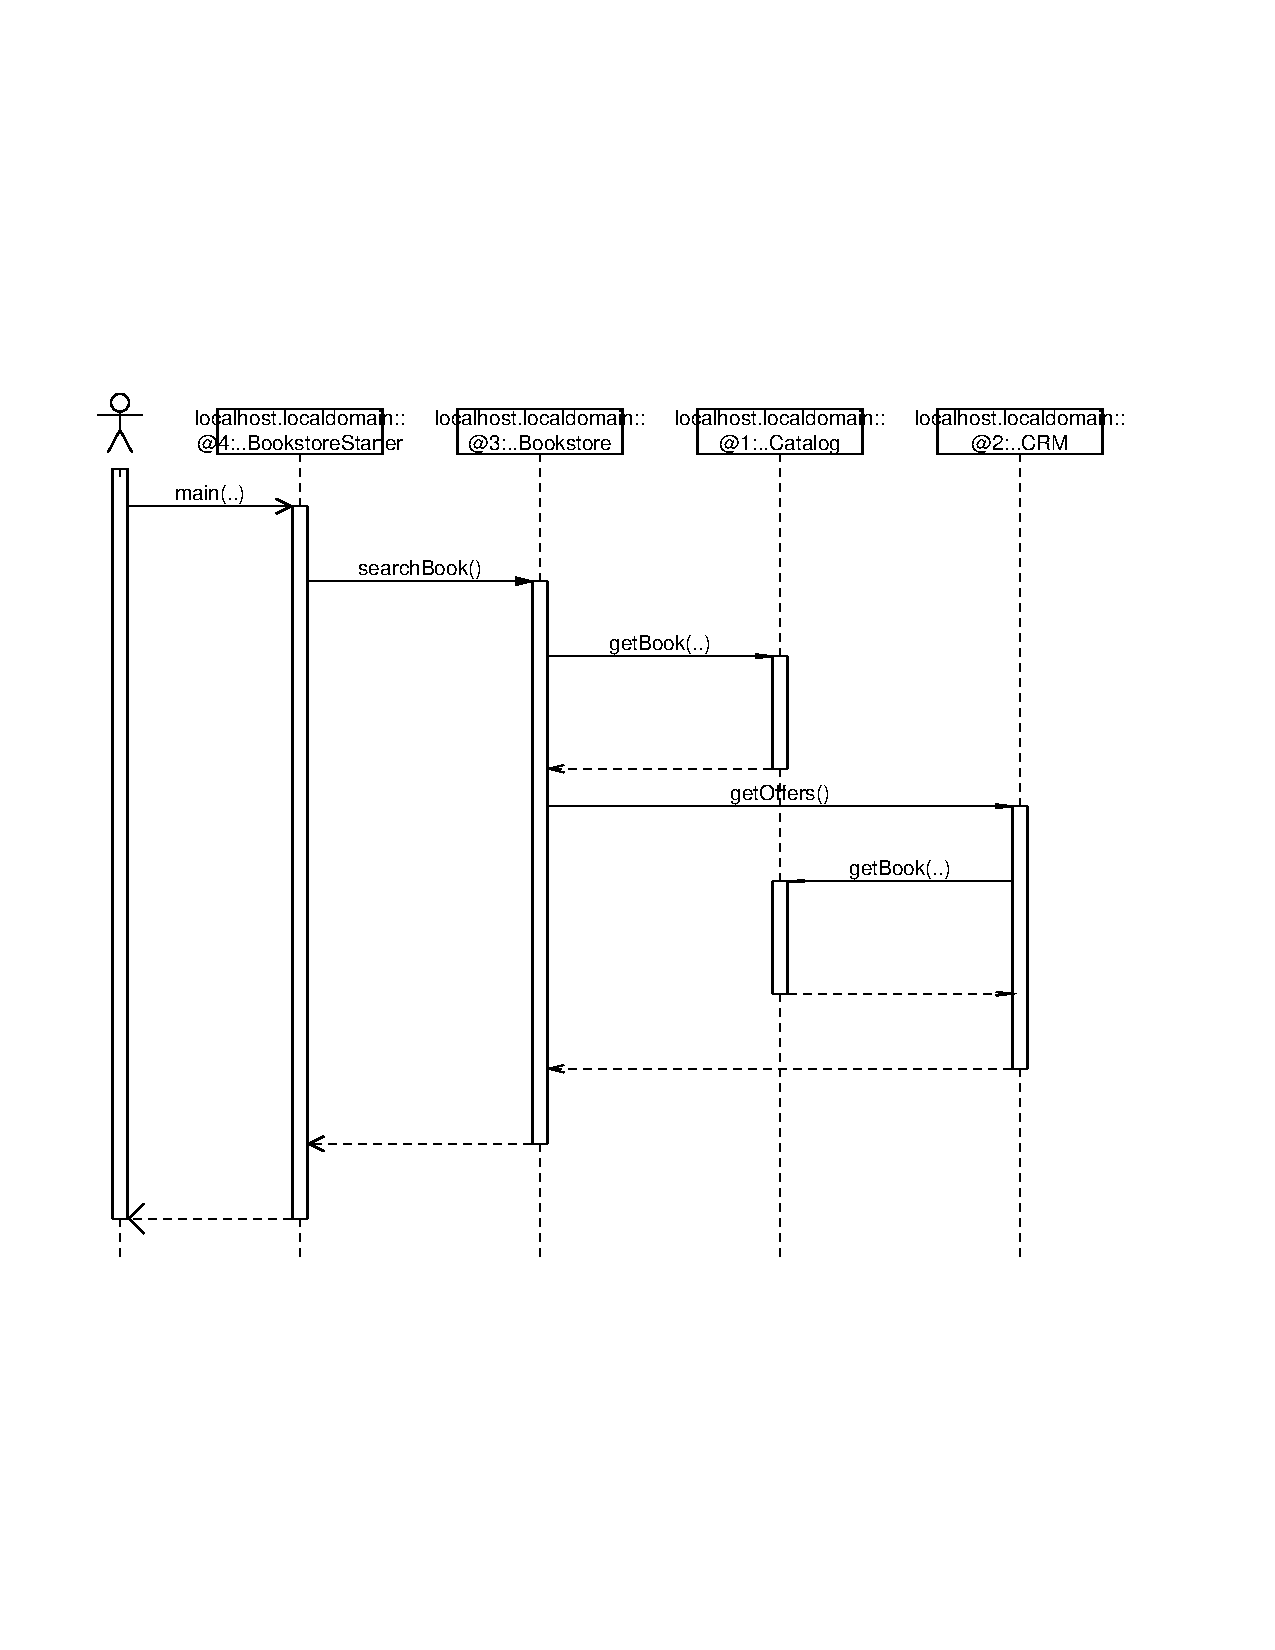
\includegraphics[height=0.5\textheight]{images/allocationSequenceDiagram}
		\caption{allocationSequenceDiagram}
	\end{figure}
	\begin{figure}[H]
		\centering
		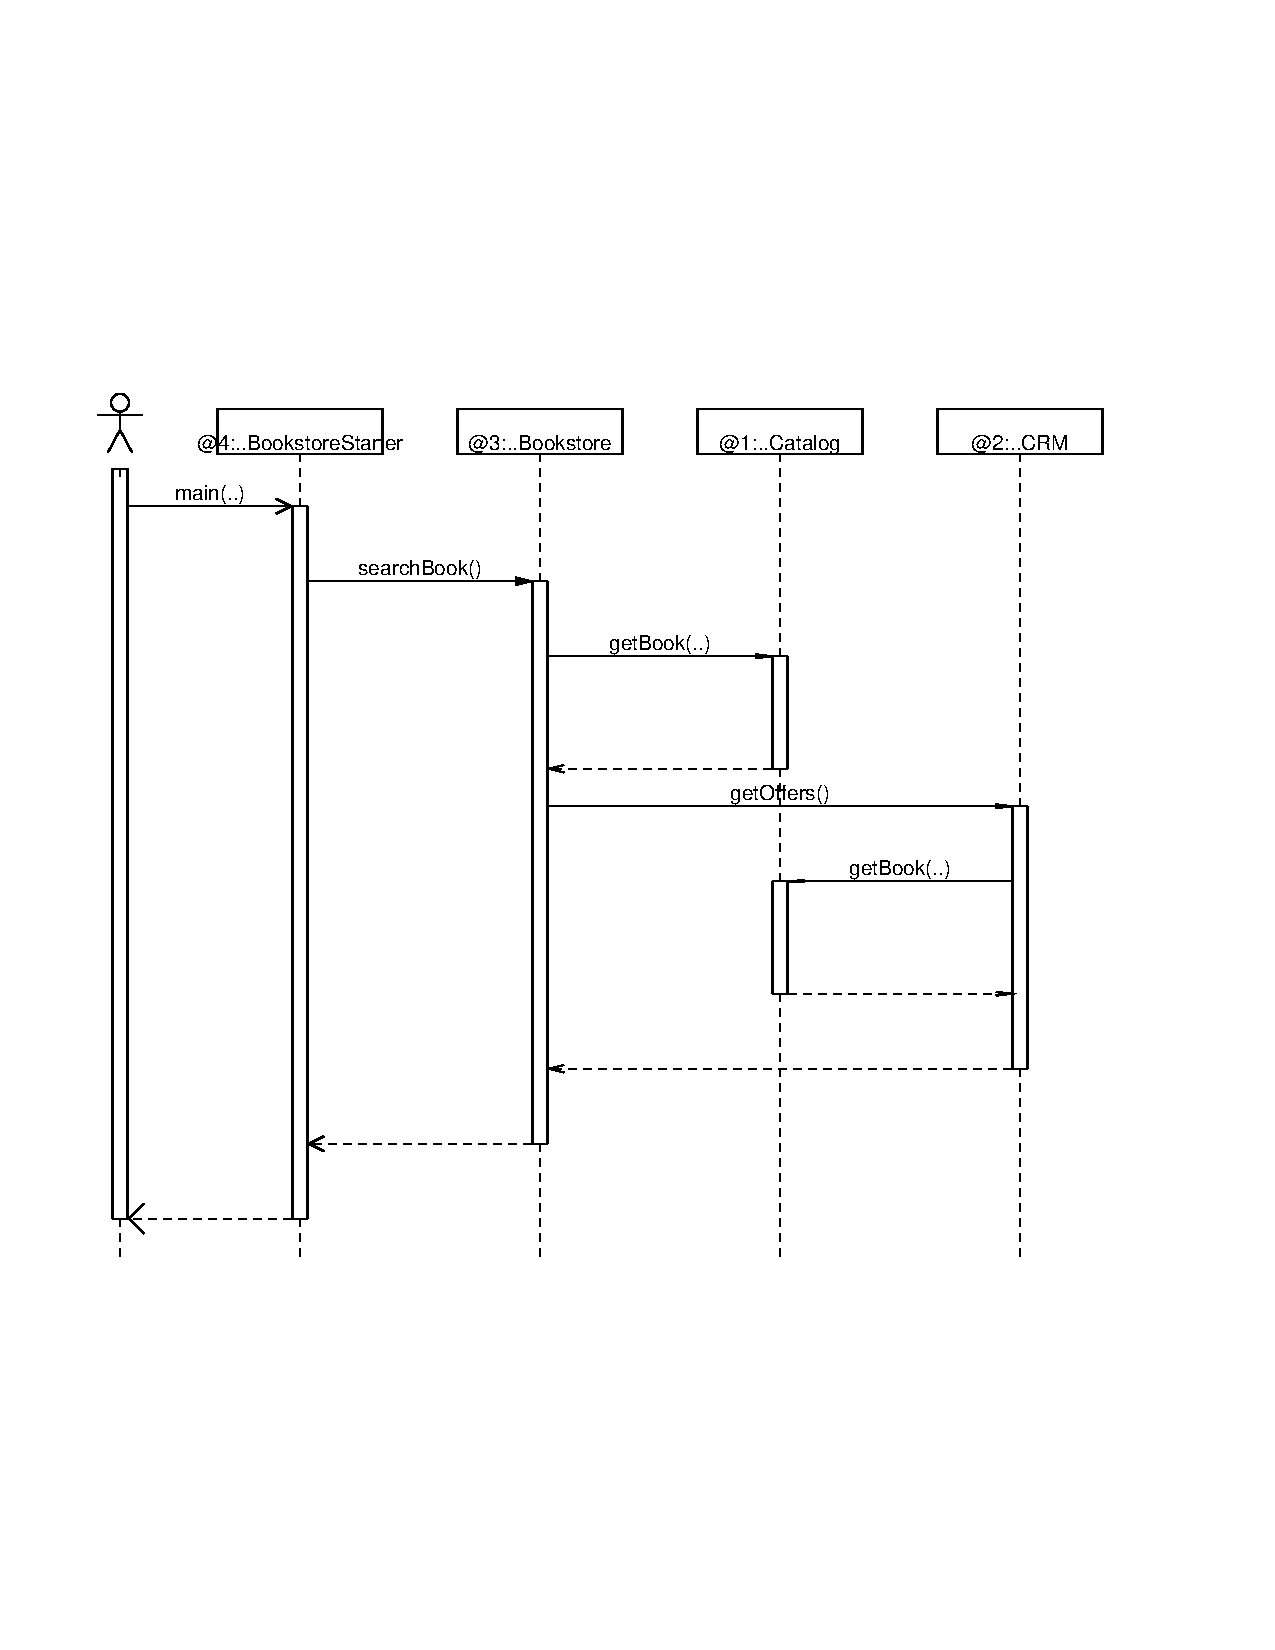
\includegraphics[height=0.5\textheight]{images/assemblySequenceDiagram}
		\caption{assemblySequenceDiagram}
	\end{figure}
	
	\begin{figure}[H]
		\centering
		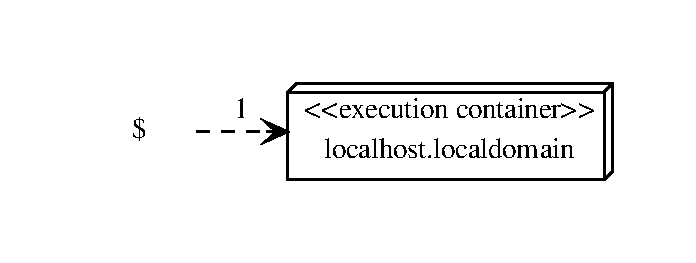
\includegraphics[height=0.5\textheight]{images/containerDependencyGraph}
		\caption{containerDependencyGraph}
	\end{figure}
  
  
\newpage
  \section{Libraries}
    The following table shows all libraries which are used by \Kieker\ and explains them briefly.
    \begin{center}
\begin{longtable}{|p{0.4\textwidth}|p{0.5\textwidth}|}
\hline 
Filename & Description\\
\hline
\hline 
commons-cli-1.2.jar & n/a\\
\hline 
maven & n/a\\
\hline 
mysql-connector-java-5.1.5-bin.jar & The library to connect to an existing MySQL database.\\
\hline 
spring-web.jar & n/a\\
\hline 
Scenario.jar & n/a\\
\hline 
sequence.pic & n/a\\
\hline 
openjms-0.7.7-beta-1.tar.gz & n/a\\
\hline 
aspectjrt-1.6.6.jar & n/a\\
\hline 
commons-logging-1.1.1.jar & n/a\\
\hline 
aspectjtools-1.6.6.jar & n/a\\
\hline 
jms-1.1.jar & n/a\\
\hline 
concurrent-1.3.4.jar & n/a\\
\hline 
servlet.jar & n/a\\
\hline 
pmd & n/a\\
\hline 
spring.jar & n/a\\
\hline 
openjms-common-0.7.7-beta-1.jar & n/a\\
\hline 
servlet-api.jar & n/a\\
\hline 
commons-pool-1.2.jar & n/a\\
\hline 
derby.jar & This library contains the necessary drivers for the Apache Derby database.\\
\hline 
commons-io-1.2.jar & n/a\\
\hline 
cxf-rt-core-2.2.6.jar & n/a\\
\hline 
jmc.jar & n/a\\
\hline 
log4j-1.2.15.jar & n/a\\
\hline 
openjms-net-0.7.7-beta-1.jar & n/a\\
\hline 
aspectjweaver-1.6.6.jar & n/a\\
\hline 
cxf-api-2.2.6.jar & n/a\\
\hline 
rabbitmq-client.jar & n/a\\
\hline 
openjms-0.7.7-beta-1.jar & n/a\\
\hline 
spice-jndikit-1.2.jar & n/a\\
\hline 
cxf-rt-bindings-soap-2.2.6.jar & n/a\\
\hline 
cxf-common-utilities-2.2.6.jar & n/a\\
\hline 
jndi-1.2.1.jar & n/a\\
\hline 
\end{longtable}
\label{tabular:libraries}
\end{center}


% \chapter{Troubleshooting}
